\documentclass{article} % For LaTeX2e
\usepackage{nips13submit_e,times}
\usepackage{hyperref}
\usepackage{url}
\usepackage{graphicx}
\graphicspath{{images/}}
%\documentstyle[nips13submit_09,times,art10]{article} % For LaTeX 2.09


\title{Formatting Instructions for NIPS 2013}


\author{
Viraj Mehta\thanks{ Use footnote for providing further information
about author (webpage, alternative address)---\emph{not} for acknowledging
funding agencies.} \\
Department of Mathematics\\
Stanford University\\
\texttt{virajm@stanford.edu} \\
\And
Meena Chetty \\
Department of Computer Science \\
Stanford University \\
\texttt{mchetty@stanford.edu} \\
(if needed)\\
}

% The \author macro works with any number of authors. There are two commands
% used to separate the names and addresses of multiple authors: \And and \AND.
%
% Using \And between authors leaves it to \LaTeX{} to determine where to break
% the lines. Using \AND forces a linebreak at that point. So, if \LaTeX{}
% puts 3 of 4 authors names on the first line, and the last on the second
% line, try using \AND instead of \And before the third author name.

\newcommand{\fix}{\marginpar{FIX}}
\newcommand{\new}{\marginpar{NEW}}

\nipsfinalcopy % Uncomment for camera-ready version

\begin{document}


\maketitle

\begin{abstract}
In this paper, we develop a reverse dictionary model that learns formal and colloquial English word definitions. Thus, given a meaning or description, our model will output predictions for the target word. We collect data from the Merriam-Webster and Oxford English Dictionaries, as well as 16 years of data from the New York Times Crossword database and the web-scraped entries at \emph{crosswordsolver.org}. Using this data, we develop a two-fold model: it can be used on formal descriptions and meanings, as well as on puzzle-oriented ones. We tune our predictions by measuring accuracy based on the top-n predictions. For the puzzle solver application of our model, we utilize the contextual information that is inherent to puzzles such as crosswords, and we provide information such as word length and random characters within the target word to improve our prediction accuracy. Through this process, we can predict words from formal meanings with an accuracy of 0.712 and determine the solutions represented by crossword clues with an accuracy of 0.631.
\end{abstract}


\section{Introduction}
Our motivation for this project stems from the idea that people often know what they want to say, but don’t always have to words to do so. We seek to address this problem by building a reverse dictionary. Essentially, users should be able to input the general meaning of the word they are looking for, and our reverse dictionary model would output predictions for this word. Such a tool would have applications in writing papers, solving crossword puzzles, and many other daily uses of the English language.

\subsection{Goal}
We will build multiple models using techniques such as BOW and LSTM that will be trained on word definitions. We will extract these definitions from dictionaries for more formal definitions, and from crossword clues for more colloquial ones. We will experiment with various models, word vector sizes, and hyperparameters to determine which scheme works best. We will measure accuracy based on the percentage of our model’s predictions that match the true word corresponding to the input definition. We will also determine a second metric for top-n accuracy, where we will measure the percentage of our model’s top n predictions that contain the true word corresponding to the input definition. From there, we will identify how to refine our model and test in which contexts it performs best.

\subsection{Applications}
Our first step in solving this problem is to understand the specific use cases that we want to target. We have 2 primary use cases: 
\begin{itemize}
\item Traditional reverse dictionary: The input for this use case is a comprehensive definition or meaning of the target word. This application is better suited for writing essays or formal literature. 
\item Crossword/word puzzle solver: The input for this use case is more cryptic or colloquial than that of a reverse dictionary. This application is better suited for solving word puzzles, such as crosswords. The input to our model for this application would differ slightly in that the crossword solver would also be provided lengths of target words and select characters within the word, since crosswords and word puzzles inherently provide this information. 
\end{itemize}

\section{Background and Related Work}
Previous research has been conducted on how to build crossword solvers and reverse dictionaries independently with NLP, but the two problems are not often combined and do not always use deep learning.
To build the crossword-solver aspect of this problem, Radev et al formed a constraint satisfaction problem using positioning of characters in words within a crossword puzzle as well as all other clues available to determine word predictions. Thus, using contextual information from an entire crossword along with word definitions and previously solved crossword puzzles, they determined confidence scores to generate predictions for solutions to entire crosswords.
Meanwhile, Hill et al addressed the reverse dictionary component of this problem using deep learning, which is more relevant to the problem we are trying to solve. They use models similar to ours, such as Bag of Words (BOW) and Long Short-Term Memory Recurrent Neural Networks (LSTM RNN’s), but train their models exclusively on dictionary data for the purpose of reversing formal word definitions. They achieved an accuracy of 0.89 through these methods. 
Thus, a new area of research would be combining these two problems into one such that we can generate a single model that can accommodate both problems: reversing both formal and cryptic or colloquial definitions.

\section{Data and Annotations}

\subsection{Datasets}
Training our model requires extensive datasets of word definitions. Finding such datasets is not difficult due to the existence of dictionaries. However, dictionaries contain exclusively formal definitions of words. Users should not be expected to input definitions with such a high degree of formality in order to obtain the word they are looking for, because that would not be a practical use case of our model. 
In order to ensure that our data includes less traditional word definitions, we scraped large datasets of crossword clues as well. While crossword clues tend to be more cryptic than traditional meanings and definitions, they incorporate more colloquial speech than dictionary definitions might. 
Thus, our comprehensive dataset includes all word definition and word pairs from the Oxford English Dictionary and Merriam Webster Dictionary, as well as 432,205 crossword clue and solution pairs from the New York Times database of crosswords from the past 16 years and \emph{crosswordsolver.org}. 
Our dictionary definitions are standard dictionary definitions pulled verbatim from accredited dictionaries. Below are a few examples of what crossword clues might look like:

\textbf{Definition}: places for mending; \textbf{True word}: sanitaria. 

\textbf{Definition}: doesn’t talk smoothly; \textbf{True word}: rasps

\textbf{Definition}: noodle-and-vegetable soup; \textbf{True word}: ramen

\subsection{Application-based Data Usage}
Our train dataset for our model includes all word definitions from the Oxford English Dictionary, and a randomized 70\% of the crossword clues from the New York Times database. Our test and dev sets vary between the two applications of our model.
For the reverse dictionary application of our model, our test set consists of all word definitions from the Merriam Webster Dictionary (a different dictionary than the one contained in the train set). It did not make sense to combine all definitions and randomly split them into train, test, and dev datasets, because some definitions would be repeated while some would not exist at all in these datasets, as all English dictionaries contain most of the same words with similar definitions. [dev set is the same as train set…?]
For the crossword solver application of our model, our dev set consists of 20\% of the crossword clues from the New York Times database, and our test set consists of the remaining 10\% of these crossword clues.
For all our data, we used the GloVe pre-trained word vectors to represent our words.

\section{Approach}
As previously mentioned, the limited research surrounding deep learning for reverse dictionary applications focuses on LSTM models. Thus, the process that we follow to find an optimal model begins with a vanilla LSTM and experiments with stacked and bidirectional LSTMs as well. Our variable parameters in each model are word vector dimensions and number of layers for LSTM models. We also added a regularization parameter to account for overfitting.

\subsection{Human Evaluation}
In the course of training and testing our various machine-learning models, we wanted insight into the actual difficulty of solving these clues as well as the type of problem-solving humans use in that process. We therefore created a small dataset randomly sampled from the test set of crossword clues for humans to attempt. We’ll cover the results later.

\subsection{Model Baseline}
To establish a baseline for the kind of results we might see when solving this problem, we first implement a Bag of Words (BOW) model, where we start with the pretrained embeddings of every word in the clue, add them together, and use a fully-connected layer also initialized to the transpose of these embeddings to predict logit word probabilities. Because BOW is primarily used to represent features of words and does not use any deep learning, it establishes a solid baseline that our deep learning model should be able to beat. We begin testing this model with 50-dimensional word vectors. An example of our top 10 predictions for two similar words are as follows:

\textbf{True word}: capital punishment
\textbf{Predictions}: high, lash, ease, capital, jail, penitentiary, shush, turmoil, inner, upper

\textbf{True word}: death penalty
\textbf{Predictions}: death, sin, remission, ill, grievous, punishment, mortal, guilty, conviction, child


While these true words have very similar meanings, the predictions vary drastically. Given a prediction in the first set, one would not necessarily associate a prediction in the second set. 
Thus, we conclude that overfitting may be occurring, since the slight difference in similar definitions is causing the model to vary drastically. To account for this, we add regularization in the form of dropout. As we saw in class, 0.5 was typically a successful dropout rate parameter, so we start with this value.
Additionally, we increase the dimensionality of our word vectors to 300 dimensions so that more information could be stored in each word embedding. The greater number of dimensions would ideally represent words more accurately by establishing more difference between words that were truly different rather than over-emphasizing difference between words that were relatively similar. 

\subsection{LSTM Models}
After implementing and studying results from the BOW model, which are discussed in the next section, we transition to building our LSTM models which we ideally want to result in stronger predictions. Our variables in these models are the dimensions of our word vectors, the number of LSTM stacked layers, and our regularization parameters to account for overfitting. 

\subsubsection{Vanilla LSTM}
For our vanilla LSTM model, we implement the most basic version of an LSTM in TensorFlow. Thus, it has only one layer, and uses 300-dimensional word vectors and a regularization parameter of 0.5 based on our results from the BOW model.
For a sample definition, “stretch out on a sofa,” for which the correct word is “loll,”, this model generates the following top 10 predictions: rest, couch, nap, chaise, bed, lounge, loll, dream, sit, and eke.
While the top 10 predictions are capturing the target word, we can see that our model is generating words such as “couch,” “chaise,” and “bed,” which are similar to the noun “sofa,” but are not similar to the entire action of “stretch out on a sofa” as the other words are. To add more depth to our model such that it can account better for parts of speech, we will build a model with more layers, as discussed in the next section.

\subsubsection{Stacked LSTM}

\begin{figure}
    \centering
        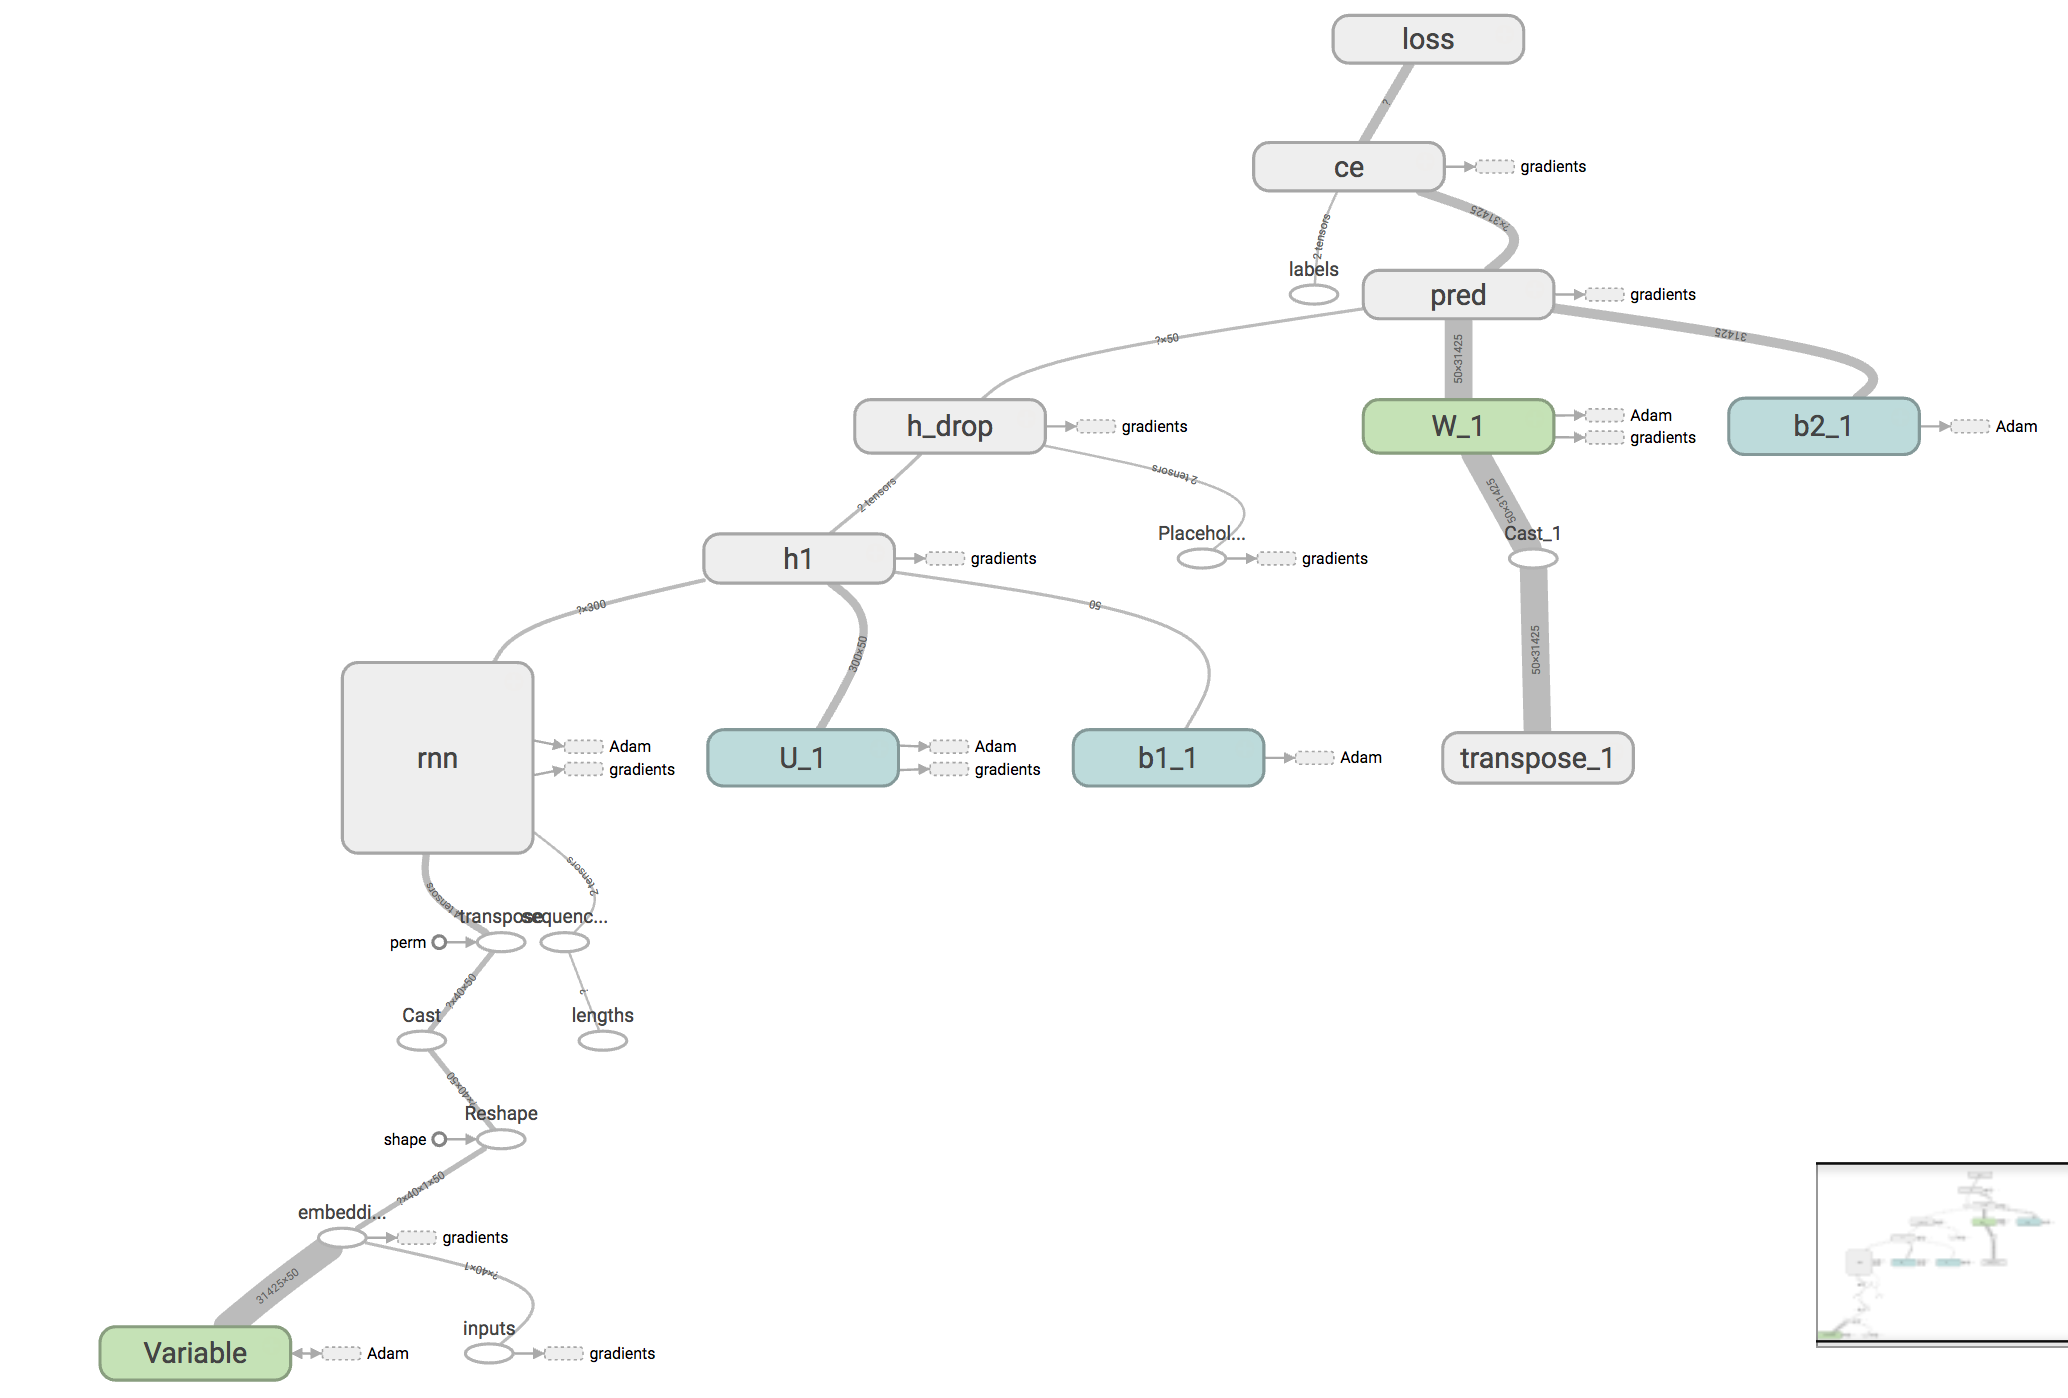
\includegraphics[width=100mm]{stacked_network.png}
        \caption{Fig 1: Model of our stacked LSTM model}
\end{figre}

This model is identical to the final version of our vanilla LSTM aside from the number of stacked layers used. Because stacked LSTM’s increase the number of layers that an LSTM has to learn information about its input, our hope in increasing the number of layers is that predicted words will account for parts of speech and tense in ways that our vanilla LSTM did not.
The predictions for “stretch out on a sofa” for this model are as follows: lounge, loll, couch, rest, nap, sleep, dream, sit, relax, unwind.
We can see that these predictions are better than the vanilla LSTM in that they caption more actions as opposed to nouns similar to sofa. Rather than “chaise” and “bed,” we instead see “relax” and “unwind,” which are more similar in meaning to our definition. 
Additionally, we can see that our loss converges relatively steadily for this model in the figure below.

\begin{figure}
    \centering
        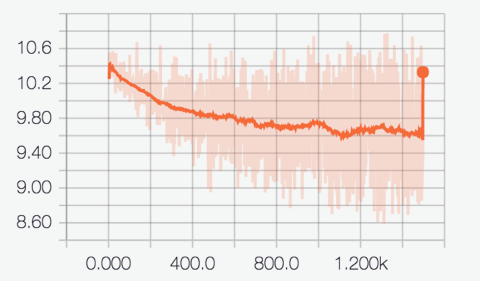
\includegraphics[width=50mm]{loss.png}
        \caption{Fig 2: Loss of stacked LSTM model in tensorflow}
\end{figure}

\subsubsection{Bidirectional Stacked LSTM}
To optimize our model further, we implement a bidirectional stacked LSTM so that our model would have more flexible input data. Since our problem is not chronologically limited and we have access to all words and definitions when building the model, bidirectionality will increase the amount of input information for each time step. Increasing the amount of data available for each prediction also helps introduce more context clues, which may help with distinguishing parts of speech and tense.  
The predictions for “stretch out on a sofa” for this model are as follows: rest, lounge, loll, sofa, relax, splay, sit, lie, nap, sleep.
As we can see, this model performs similarly to the simply stacked LSTM, outputting only one word that more closely identifies with the meaning of “sofa” than with the meaning of “stretch out on a sofa”; that word happens to be “sofa” itself in this case, which is inherently closer to “sofa” than words generated from previous models, such as “couch” or “chaise.”

\section{Model Limitations}
The majority of our model’s limitations come from our datasets. When a person is using a reverse dictionary, the type of input they provide to our model is unpredictable: it could be a sentence with a blank word, or a colloquial representation of the word in question, or a comprehensive definition or meaning. It is hard to account for this type of unpredictability given our datasets. Dictionary definitions provide a holistic coverage of comprehensive and structured inputs. However, even crossword clues do not offer the best representation for colloquial definitions because crossword clues are more cryptic than colloquial. 
Colloquial definitions are likely to be the most frequent input to our model, since people do not speak in the same formal format that a dictionary is written. Additionally, our model accounts only for denotation as opposed to connotation. In colloquial word definitions, people often associate meaning with connotation. Thus, our model is limited because it is trained on a relatively specific input dataset compared to the types of definitions and meanings that it might encounter in an application context.

\section{Experiments and Analysis}

\subsection{Human Analysis}
We had n=19 human subjects, with an average accuracy of 8.4\%. Our sample of human problem solvers included several Stanford faculty, a Jeopardy contestant, and undergrads from a variety of fields. The best human scorer was at 12\% accuracy, so we feel confident that our models are vastly outperforming even expert humans.
Qualitatively, it seems that for the clues that human problem-solvers get correct they usually leverage a more bag-of-words approach than a sequential one to reach the clue. For example, ‘childrens block company’ quite easily maps to Lego irrespective of the permutations of the words. These are the vein of clues that humans do well on. We notice similar trends in our models, with the bag-of-words family only outdone by our most advanced LSTM models.

\subsection{Experimental Results}
We evaluate our models based on accuracy metrics that we calculate for all four models listed above, on both 50-dimensional and 300-dimensional word vectors. Additionally, evaluations are done separately for crossword clue predictions and dictionary definition predictions.
Our first accuracy metric is ratio of correctly predicted words to total number of input word definitions. We measure accuracy on both our dictionary test set and our crossword clues test set to keep the accuracies of the two applications of our models separate, as discussed in Section 3.

\begin{figure}
    \centering
	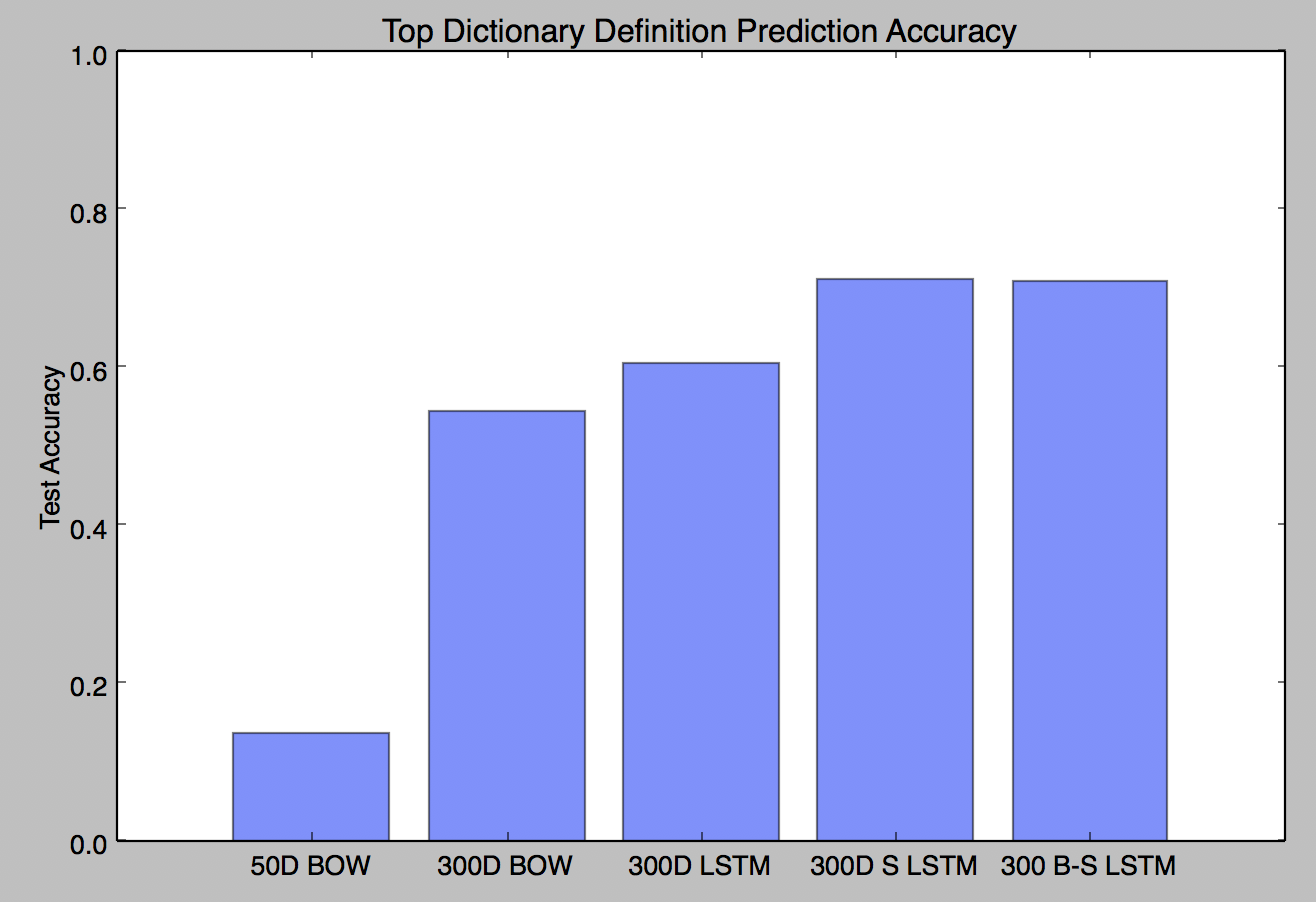
\includegraphics[width=50mm]{REAL_topdictdef.png}
	\caption{Fig. 2: Accuracy of top prediction for the true word corresponding to the dictionary definition.}
\end{figure}

\begin{figure}
    \centering
	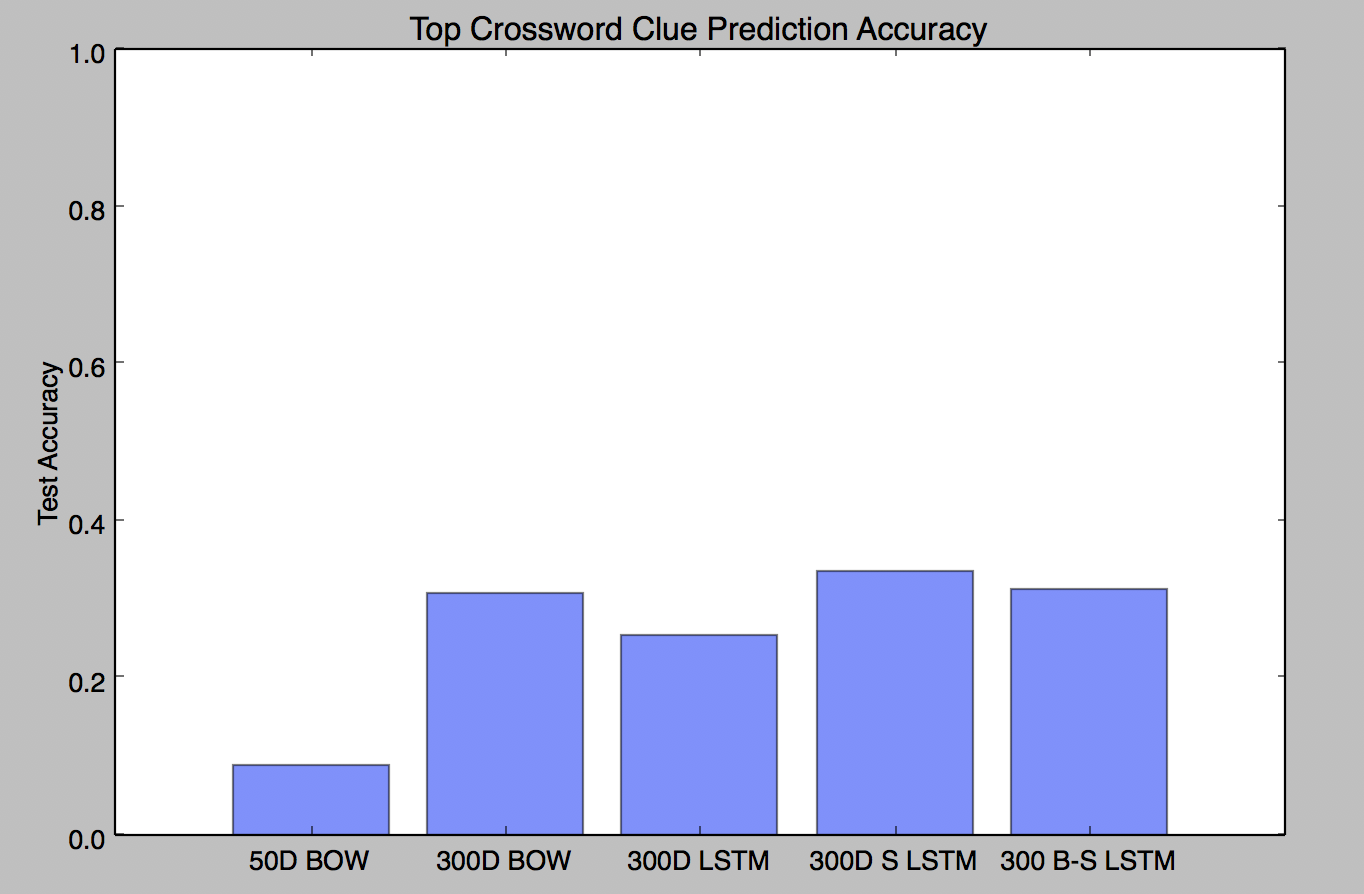
\includegraphics[width=50mm]{REAL_topcrossclue.png}
	\caption{Fig. 3: Accuracy of top prediction for the true solution corresponding to the crossword clue.}
\end{figure}

Since these accuracy values are not very high for crossword clues, we then reveal the top 10 predicted words for crossword clues as opposed to simply the top predicted word for each definition, so that we can determine whether our model was in the ballpark for a larger number of words than it appeared. We redefine our accuracy metric to be the ratio of top 10 predicted words that contain the correct target word to the total number of input word definitions. The accuracies are as follows:

\begin{figure}
    \centering
	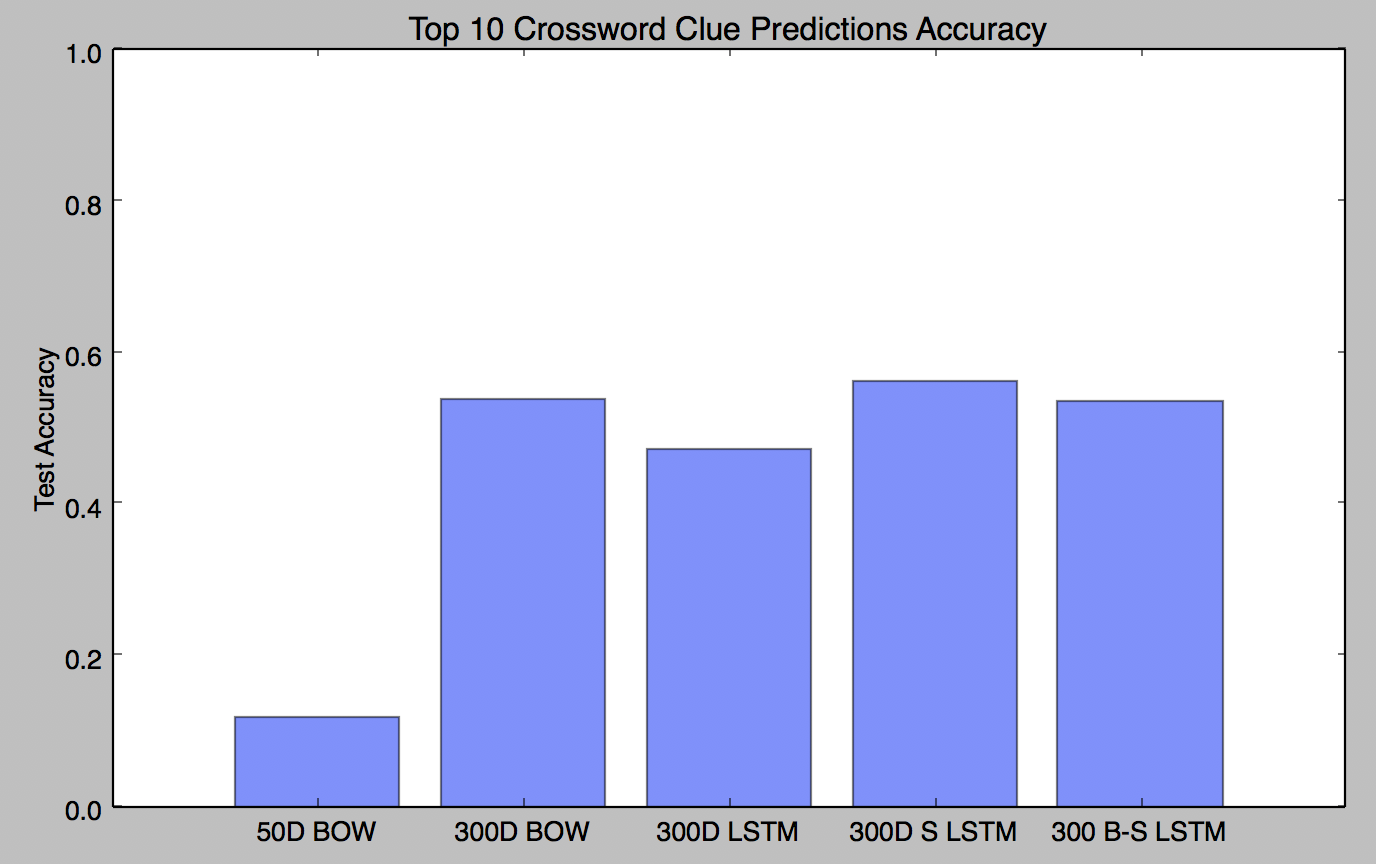
\includegraphics[width=50mm]{top10cross.png}
	\caption{Fig. 4: Accuracy of top 10 predictions for the true solution corresponding to the crosswordclue.}
\end{figure}

These accuracy values are significantly better than the prior metric. We then see that adjusting our evaluation metrics can refine our model’s predictions better than adjusting our actual model can. For the crossword application of our model, we develop two new accuracy metrics to do so based on the extra information that is inherent to crosswords:
Provide the length of the correct word with the word definition, so that we can iterate through the top n word predictions and return the first word of the correct length.
Provide a random character and its index from the correct word with the word definition, so that we can iterate through the top n word predictions and return the first word with this character at the given position. 
This approach results in the following accuracies for our crossword clue test set, where n=10:

\begin{figure}
    \centering
	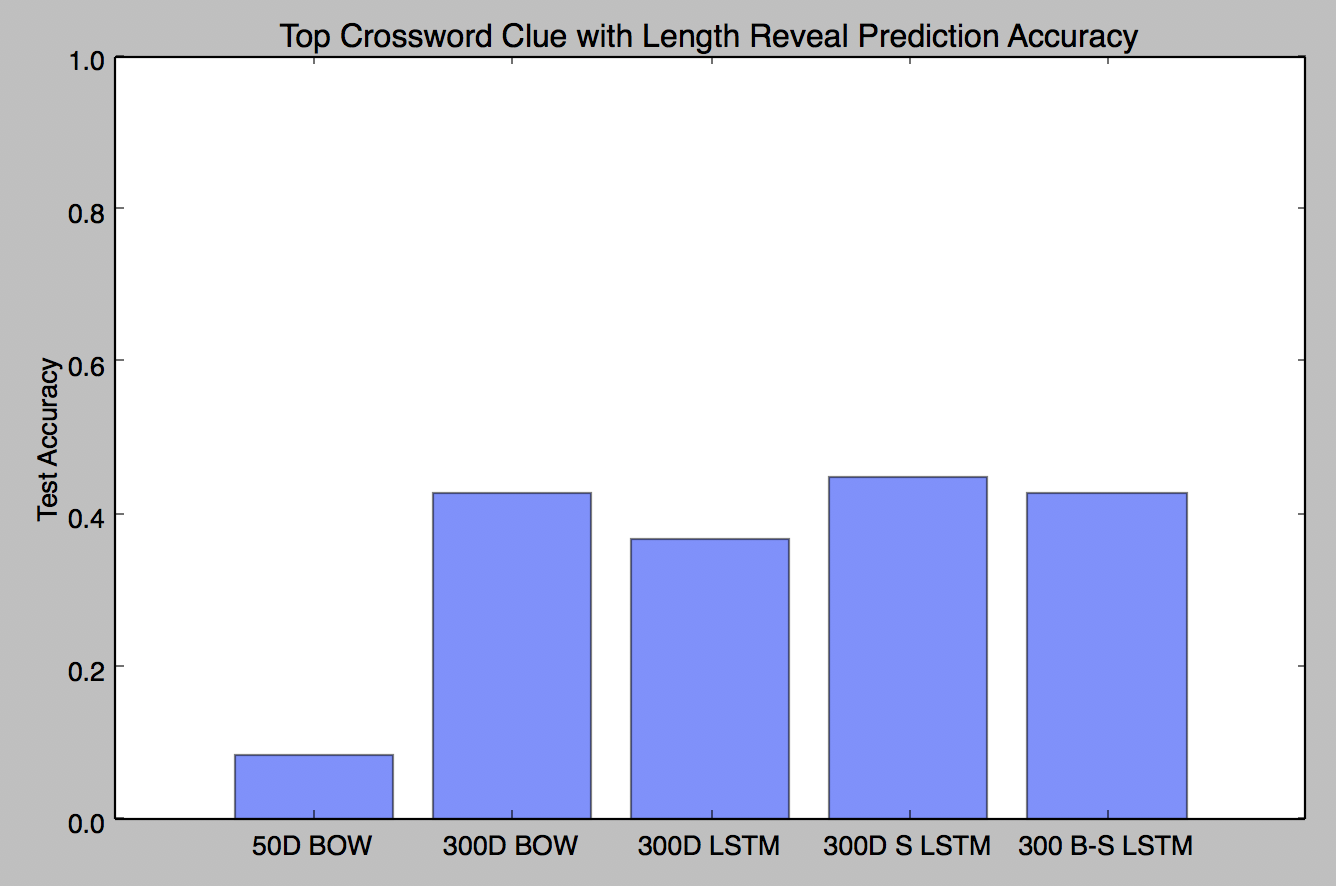
\includegraphics[width=50mm]{top10len.png}
	\caption{Fig. 5: Accuracy of top the prediction for the true solution corresponding to the crossword clue given the true solution length.}
\end{figure}

\begin{figure}
    \centering
	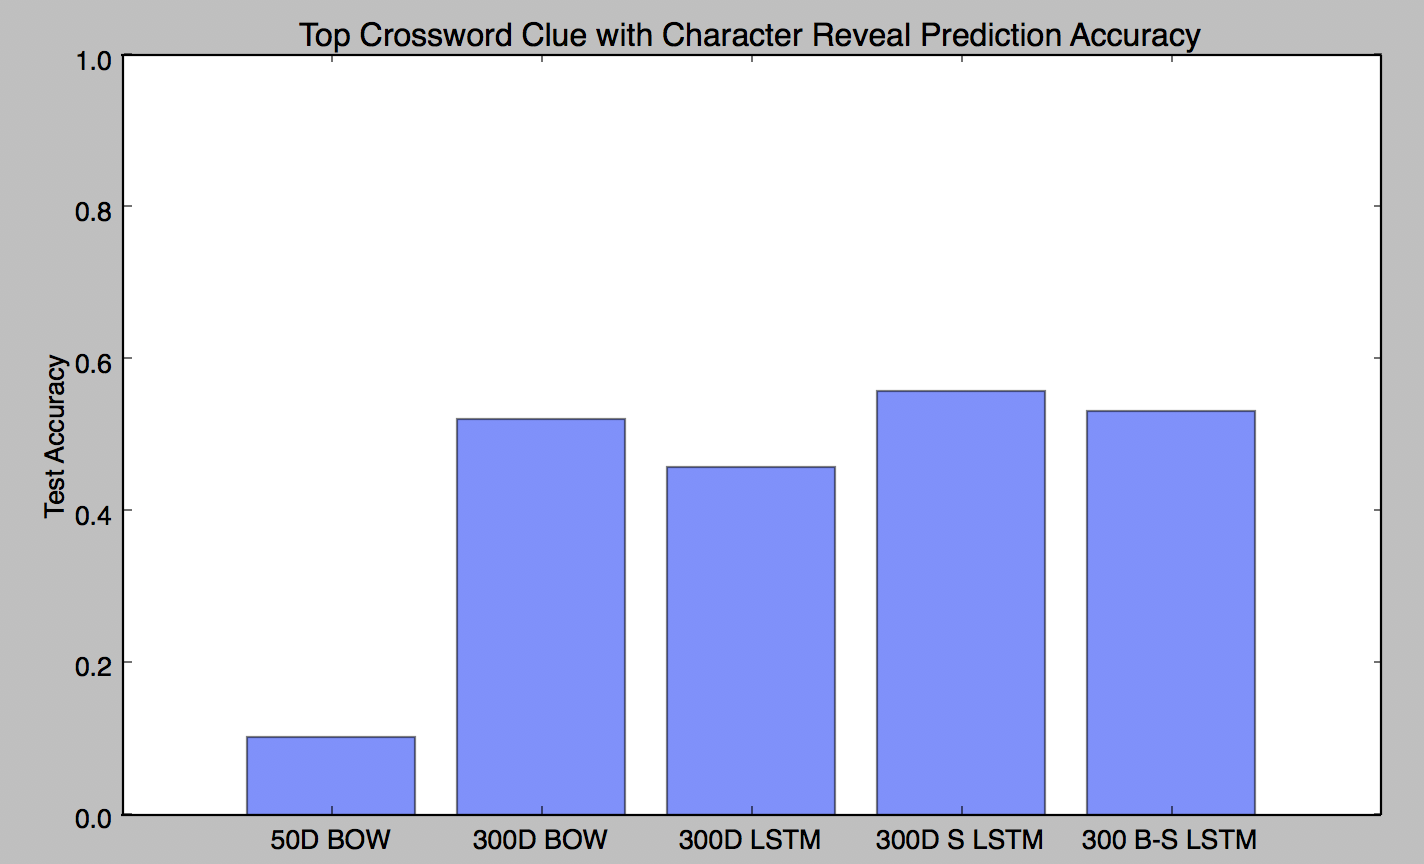
\includegraphics[width=50mm]{top10char.png}
	\caption{Fig. 6: Accuracy of the top prediction for the true solution corresponding to the crossword clue given a random character in the true solution.}
\end{figure}

Since many of these accuracies were less than the top 10 general predictions, which was contrary to our hypothesis, we expanded our sample size to n=50 to improve our accuracy:

\begin{figure}
    \centering
	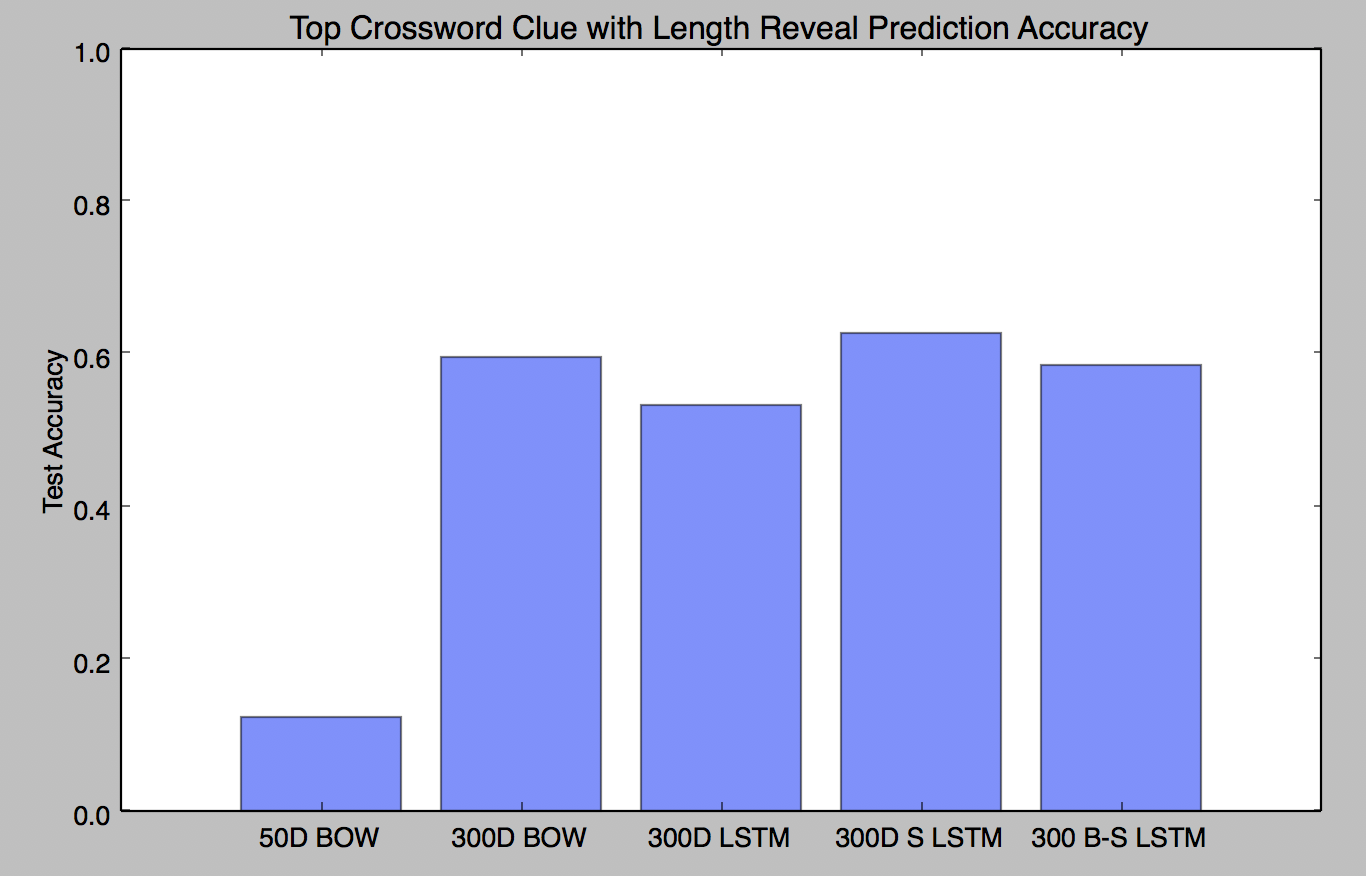
\includegraphics[width=50mm]{top50len.png}
	\caption{Fig. 7: Accuracy of the top prediction for the true solution corresponding to the crossword clue given the true solution length.}
\end{figure}

\begin{figure}
    \centering
	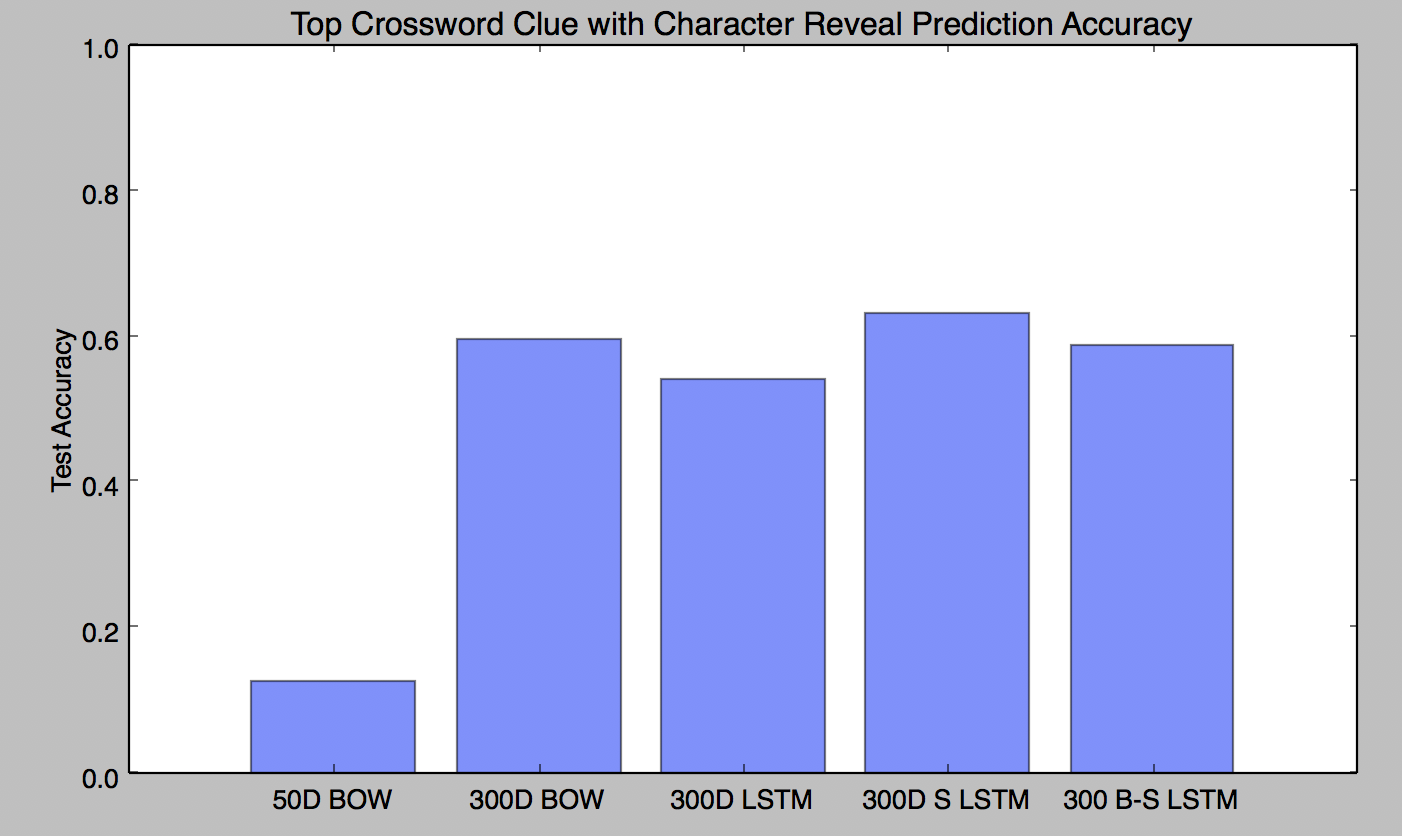
\includegraphics[width=50mm]{top50char.png}
	\caption{Fig. 8: Accuracy of the top prediction for the true solution corresponding to the crossword clue given a random character in the true solution.}
\end{figure}


The best accuracy we achieved for dictionary definitions (and therefore the more formal reverse dictionary application of our model) was 0.712 with the 300-dimensional stacked LSTM model. The best accuracy we achieved for crossword clues (and therefore for the puzzle solver application of our model) was 0.631 with the 300-dimensional stacked LSTM model using character reveal during evaluation. 
Evidently, our model works better on dictionary definitions than on crossword clues. This is to be expected given our discussion about our model’s limitations and the fact that it is better trained to handle formal word definitions. 


\section{Conclusion}
In designing and then in pursuing this project we were simultaneously pursuing a variety of goals. We succeeded to varying degrees in achieving them with the flexible architecture we pursued. In particular, we are pleased with our performance on the challenging problem of solving crossword clues without additional information, in which we vastly outperformed humans. The main takeaway of this result is that we have found a reasonable neural representation of the language which encodes the knowledge advantage a neural system gets in training. Colloquially, after feeding our network a dictionary, we can now be convinced of the digestive process as well.

We are also pleased that our postfix modifications to include additional information provide modest increases in performance, to the point that it might be reasonable to expect our system to bootstrap itself into solving full crosswords. 

While Hill et al achieved an accuracy of 0.89 on their dictionary definition-specific model and we only achieved 0.71 on our model for the reverse dictionary application, our model’s accuracy is likely lower because it includes crossword clues in the training set as well as dictionary definitions in order to accommodate the puzzle solver application of our model. Though our accuracy on dictionary clues is far from perfect, our example results show that the system is typically in the right ballpark on finding the word and might be useful for finding related words. 

\subsection{Future Directions}
We see a few directions for future research in the area. First, it could be instructive to devise methods of combining this model with search- or constraint-based models to attack the task of solving full crosswords. In a model like that, this algorithm would be a method of finding and ranking candidates for a search or CSP module that would address the more global picture of the crossword. It could also be interesting to try and design a differentiable architecture to allow such a system to be trained end-to-end.
Another potential direction for future research is in building character-by-character models to  predict each successive character of  a correct answer. These architectures could potentially include the added crossword information to the character-prediction process. We strongly considered implementing one of these for our current research but ultimately decided that it was not in line with our goal of building the dual-purpose system we currently have.


\section*{Acknowledgments}

Use unnumbered third level headings for the acknowledgments. All
acknowledgments go at the end of the paper. Do not include 
acknowledgments in the anonymized submission, only in the 
final paper. 

\section*{References}

References follow the acknowledgments. Use unnumbered third level heading for
the references. Any choice of citation style is acceptable as long as you are
consistent. It is permissible to reduce the font size to `small' (9-point) 
when listing the references. {\bf Remember that this year you can use
a ninth page as long as it contains \emph{only} cited references.}

\small{
    
}

\end{document}
